% ==================================================
% CHAPTER 6: Comparing cosmic muon and x-ray relative strip position offsets %
% ==================================================

\chapter{Comparing cosmic muon and x-ray relative strip position offsets}
\label{chap:comparison}
% Edit count: Lia - 1, Brigitte - 0

The goal was to validate the local offsets extracted from the x-ray data with cosmics data. The complication was that the x-ray dataset provided absolute local offsets while the cosmics dataset provided relative local offsets, which could not be compared directly. The solution was to analyze the x-ray data in the same relative coordinate system as the cosmics data. The methods and results of the comparison are presented here.

% --------------------------------------------------
\section{Method for comparing x-ray and cosmics data}
% --------------------------------------------------
%TODO : determine if the description of equation 1.1 is suitably general enough to describe the x-ray data

The measured x-ray beam profile centers were systematically affected by local offsets in the same way as the mean cosmics residuals, as modeled by equation \ref{eqn:local_translation}. Therefore, if a 2-layer track is abstracted from the beam profile centers on each layer and the residual calculated on a third layer, that residual should match the local mean cosmics residual. 

The track is "abstracted" because a so-called "beam profile center" is actually the Gaussian mean of all selected mean cluster positions recorded during the x-ray data taking period. Abstracting a track was necessary because the x-rays cause signal in the chamber via the photoeffect so there were not individual "x-ray tracks" to record. In fact the x-ray data was collected separately for each layer. Nonetheless, since the effect of local offsets on the beam profile centers was the same the difference in algorithm between x-ray and cosmics analysis was allowed. 

For each x-ray survey position, the x-ray residual was calculated for all possible tracking combinations (which required an x-ray beam profile on at least three layers). The position of the x-ray residuals are shown as black dots over figure~\ref{fig:res_mean_th2_L2_F13} and \ref{fig:res_mean_th2_L4_F13}. Note that the mean of cosmics residuals around the x-ray points were calculated in bins exactly centered on the nominal x-ray gun position, unlike in figure~\ref{fig:res_mean_th2}.

%---------------------------------------------------
\section{Assessing correlation}
%---------------------------------------------------
\label{sec:assessing_correlation}
Scatter plots of the x-ray and mean cosmics residuals for two sample quadruplets in figures~\ref{fig:correlation} and \ref{fig:no_correlation} reveal the degree of correlation between the datasets.

\begin{figure}
    \centering
    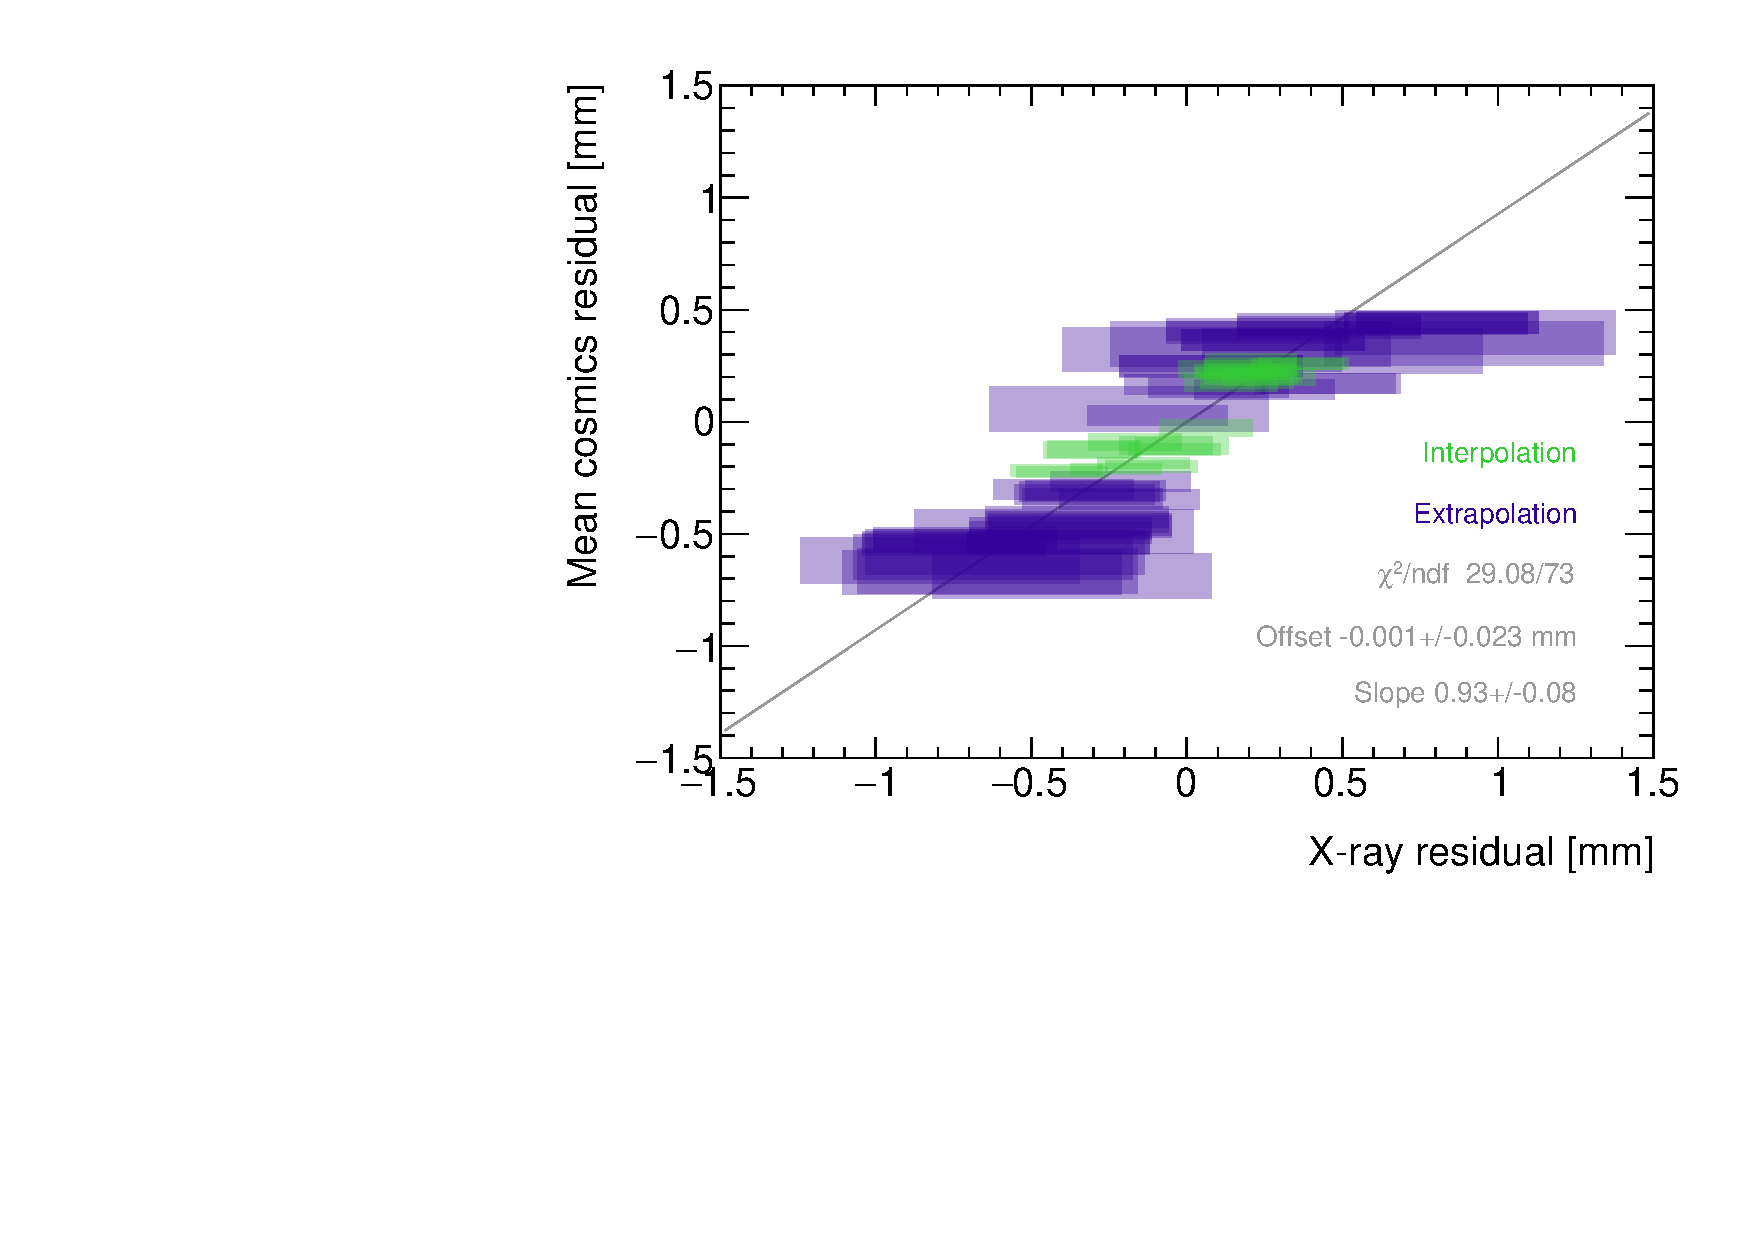
\includegraphics[width = \textwidth]{figures/figure_QL2P11_3100V_2021-08-05_QL2P11_local_cosmic_and_xray_data_correlation_plot.pdf}
    \caption{Correlation plot between x-ray and cosmics residuals for all tracking combinations for QL2.P.11. Each rectangle is centered on an x-ray and mean cosmics residual pair. The width of the rectangles in $x$ and $y$ are the uncertainty in the x-ray and mean cosmics residual respectively. A printer-friendly version of this plot is available in appendix~\ref{appendix:print}.}
    \label{fig:correlation}
\end{figure}

First, the fitted slope and offset in figure~\ref{fig:correlation} show that the two QL2.P.11 datasets are correlated. However, the magnitude of the uncertainties in the x-ray residuals is large (up to half a millimeter) since it comes from propagating the \SI{120}{\micro\meter} uncertainty in the beam profile centers. The large uncertainty set a limit on the sensitivity of the analysis, for if the absolute value of the x-ray residuals of a quadruplet were smaller than the x-ray residual uncertainties, no conclusion about the correlation could be drawn, like for QL2.P.8 (figure~\ref{fig:no_correlation}).

\begin{figure}
    \centering
    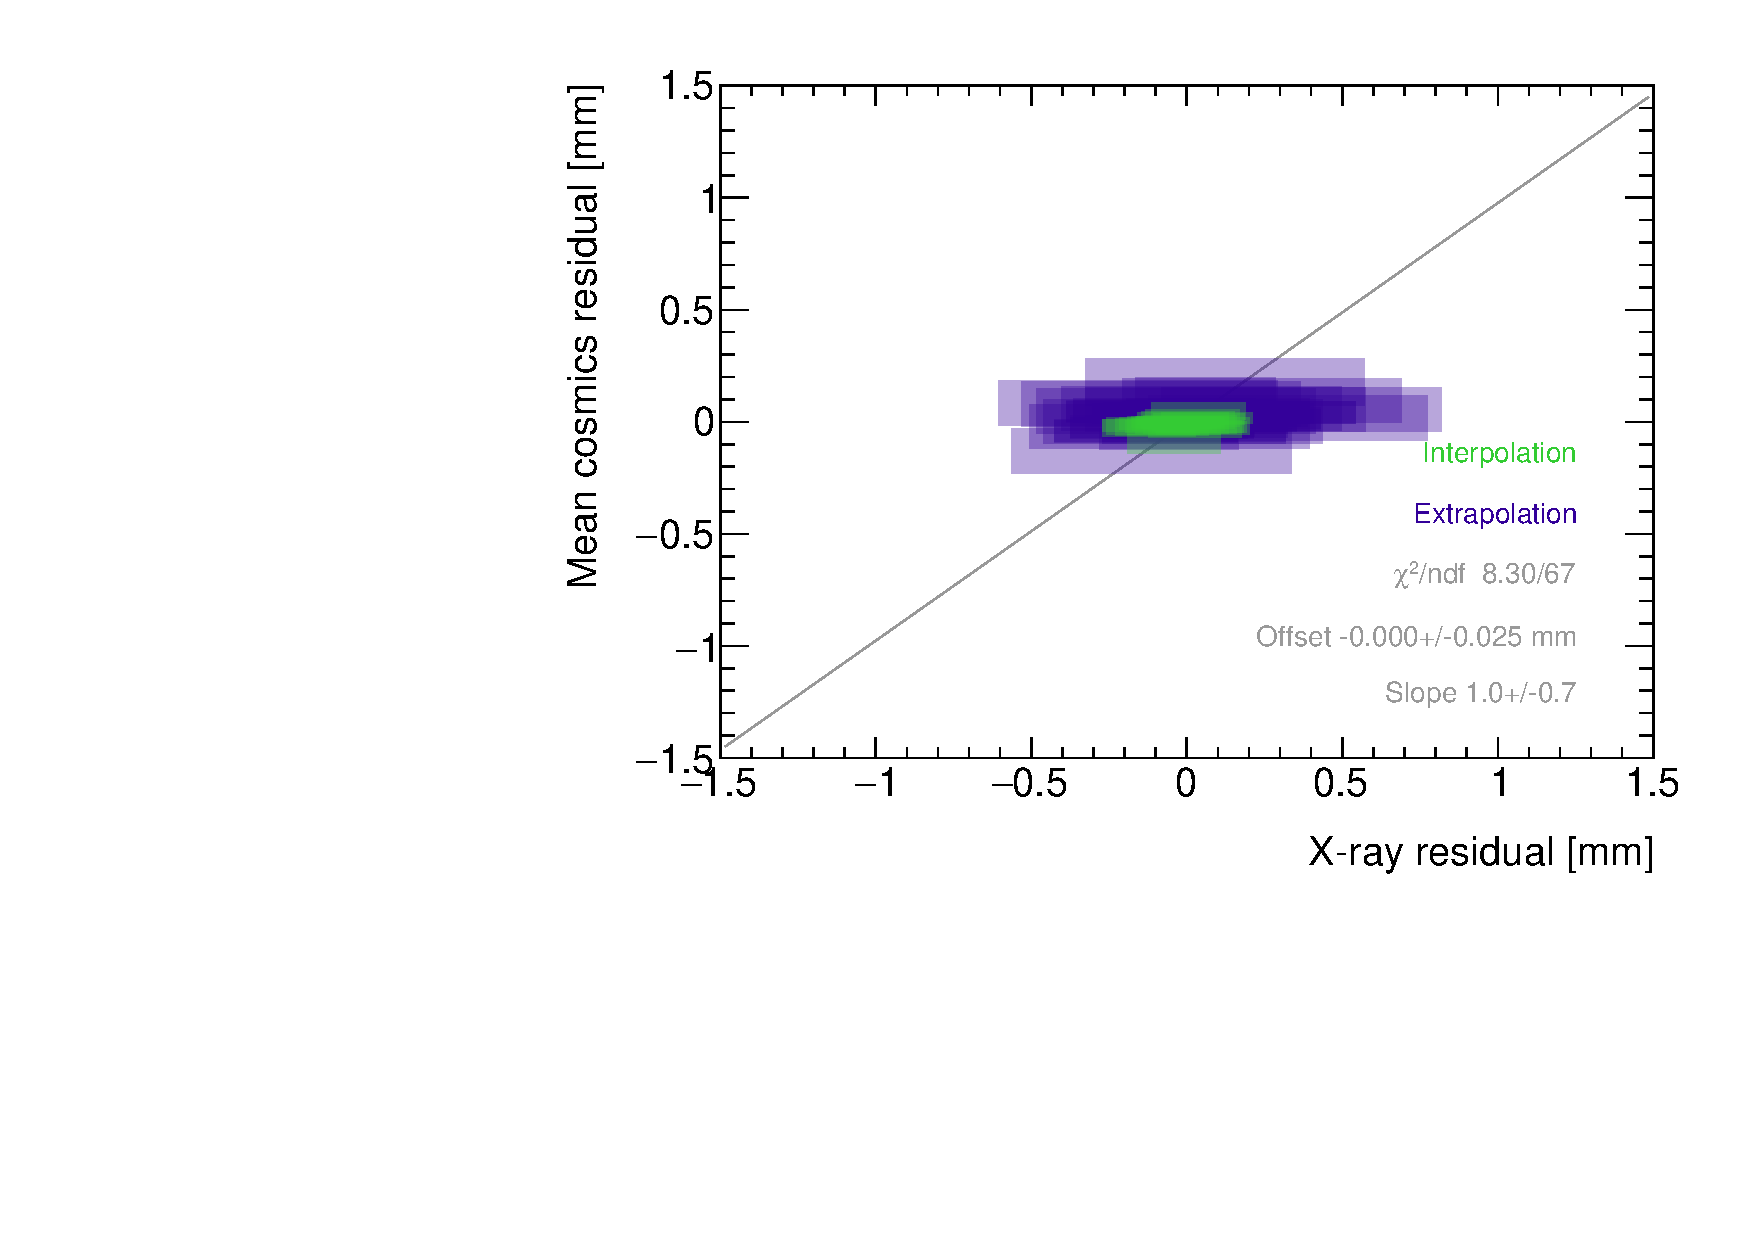
\includegraphics[width = \textwidth]{figures/figure_QL2P08_3100V_2021-08-16_QL2P08_local_cosmic_and_xray_data_correlation_plot.pdf}
    \caption{Correlation plot between x-ray and cosmics residuals for all tracking combinations for QL2.P.8. Each rectangle is centered on an x-ray and mean cosmics residual pair. The width of the rectangles in $x$ and $y$ are the uncertainty in the x-ray and mean cosmics residual respectively. A printer-friendly version of this plot is available in appendix~\ref{appendix:print}.}
    \label{fig:no_correlation}
\end{figure}

Several quadruplets were tested for each quadruplet construction geometry built in Canada: QL2P, QL2C, and QS3P. Each quadruplet fell into one of the two categories: residuals large enough to see a correlation, or residuals too small to see a correlation. Since the x-ray and mean cosmics residuals were measures of the relative local offsets between the layer of a quadruplet and the two reference layers, quadruplets with the most relative misalignment had the largest range of residuals. So, the correlation plots were an easy visual way to identify quadruplets with large relative misalignments.

There are three patterns in the residuals on the scatter plot explained by geometry. First, for both datasets the uncertainty in the extrapolated track residuals were larger than the interpolated track residuals because of the extrapolation lever arm. For the x-ray residuals, the effect of the lever arm on the uncertainty was direct since the residual was calculated from a single abstracted track; for the cosmics residuals it was the widening of the residual distribution on the layer of interest due to the extrapolation lever arm that increased the statistical uncertainty in the fitted mean of residuals. Second, residuals calculated through extrapolation tend to be larger because the extrapolation lever arm can produce more extreme values. Third, the pattern of points in figure~\ref{fig:correlation} is slightly mirrored. This is expected since the residuals calculated for a given set of three layers are geometrically correlated. 

The correlation of the cosmics residuals with the x-ray residuals alone does not validate the method; all the studies in described in appendices~\ref{appendix:statistics} and ~\ref{appendix:systematics} demonstrate its robustness. The analysis could be validated externally by comparing the mean cosmics residuals to the relative misalignment parameters calculated using \package{tgc\_analysis/MatrixMethod}~\cite{lefebvre_tgc_analysis} and JOHN FLORES CHI2 METHOD.

% --------------------------------------------------
\section{Limitations}
% --------------------------------------------------
The most important limit on measuring the degree of correlation between the x-ray and cosmics residuals was the uncertainty on the x-ray residuals, which stemmed from the systematic uncertainty in the x-ray beam profile centers~\cite{lefebvre_precision_2020}. The method was limited primarily by the sTGCs' poor x-ray position resolution, since x-rays do not create real tracks anyways. 

The analysis of certain quadruplets was also limited by the availability of data. Sometimes, less than three layers were surveyed for a given x-ray gun position so no residuals could be calculated. Too few x-ray residuals prevented the analysis from detecting a significant correlation. Often, the analysis of smaller quadruplets suffered as a result because they had fewer alignment platforms, and hence gun positions, on their surfaces. In addition, the analysis was limited to certain quadruplets. The wedges constructed the earliest (typically small wedges) were surveyed when the method was still being designed and so have limited x-ray residuals calculated from beam profiles of lower quality. Also, not all cosmic muon test sites had enough front end electronics to collect data on three layers simultaneously, which is the minimum required to be able to calculate residuals.

Nonetheless, the comparison of x-ray and cosmics residuals was really to confirm the x-ray method's ability to measure local offsets with an independent dataset; the analysis of quadruplets with relative misalignments large enough to detect a correlation achieved this goal.
